This document concludes the 12th HGSFP Winter School that took place at
the University Center in Obergurgl from 16th to 20th of January 2019. In
total, 52 graduate students from Heidelberg and 10 lecturers participated
in the five-day event. The aim of the Winter School was to give students
the opportunity to get insights into other research fields in
Heidelberg apart from their own field. In the course of this, one of the
focal points was the scientific exchange between the students
themselves and students and lecturers in a friendly atmosphere. To this
end, we organized a scientific programme consisting of 10 lectures given
by speakers from Heidelberg and other universities and two poster
sessions with elevator talks (see Appendix A).


\section*{Participant Selection}
As expected, we received more applications for the school than spots were available. We therefore had to select participants from the pool of applicants, which we wanted to perform as fair as possible. We felt it was important to be both transparent about and accountable for our selection. For this reason, we imposed a selection algorithm, laid open the complete procedure (with anonymized data)\footnote{https://github.com/matiscke/HGSFPschoolParticipantSelection}, and explain what decisions went into the selection. In the following, we give an overview on how we selected the participants for the HGSFP winter school 2019.

\subsection*{Asking The Right Questions}
Designing the application form was perhaps the most difficult task, and it is at this stage that conference organizers will already want to put serious thought into the goals of the workshop and the ideal mix of participants to achieve those goals. It should be obvious, but you will only be able to include categories in your selection that you actually ask for.

\subsection*{Pre-selection}
Excluding speakers, we have 52 spots for the meeting. Our participant selection proceeded in two parts. In the first part, we rejected candidates outright who were either (1) duplicate entries or (2) candidates who had informed us that they would not be able to come. Two spots were reserved for the HGSFP representatives. Finally, we pre-selected the organizing committee, who needs to be present at the school. Thus, a total of 8 participants (6 organizers, 2 representatives) were pre-selected. We then anonymized our applicant pool by replacing names and other identifying information with a unique identifier. 

For the remaining 52 - 8 = 44 slots, we used the software \texttt{entrofy} to optimize our participant set based on a set of well-defined criteria on which the organizers agreed. It's worth noting here that this discussion took place before performing the selection, which then depended entirely on the goals for the selection and was independent of the input data set. 

\subsection*{Target Distributions}
The targets define the fraction of participants in the final output set who share the same value of a property (e.g. 25\% of participants should be affiliated with the HGSFP branch "Fundamental Interactions and Cosmology"). The target fractions must sum up to be smaller or equal to 1.0 for each category. If the target fractions sum to a value smaller than one, the algorithm will try to fill up categories to at least the given fractions, and will ignore that category for the rest of the optimization procedure. The resulting mix of participants in the final set for this category will thus be a combination of the input fractions and the distribution in the input sample, conditioned on the constraints set by the remaining categories. Below, we will go through each category one by one and lay out our reasoning for the categories chosen. The justification for our choices is an abbreviated version of a longer discussion the organizing committee had before starting the selection procedure. We should note at this point that there is no "correct" way to choose target fractions; the target fractions must necessarily always be a function of the objectives and goals of the workshop, as defined by the organizers.

\subsection*{Selection Goals}
Broadly, the goals we defined for the HGSFP Winter School 2019 for participant selection are the following:
\begin{itemize}
	\item enable every HGSFP student to attend one winter school during their PhD:
	\begin{itemize}
		\item[$\Rightarrow$] strongly favor applicants that have not attended a HGSFP winter school before
		\item[$\Rightarrow$] favor applicants that are longer into their PhD (since the clock is ticking...)
	\end{itemize}
	\item Reflect the student numbers of the different HGSFP branches
	\item Increase the participation of underrepresented minorities (in our case this translates to an effort for gender equality)
\end{itemize}
~\\
\textbf{HGSFP branch}\\
For the branch attribute, we aim to reflect the distribution of the overall branch affiliation

~\\
\textbf{Previous Winter School Attendance}\\
Derived from our top requirement, the acceptance of applicants with previous attendance of a winter school should be an exception. We decided if we allow previous attendees at all based on the oversubscription of the school. The latter was not very high, we therefore decided to accept applicants with previous attendence only via the waiting list. We enforce this criterion further below and do not solve for this parameter.

~\\
\textbf{Gender Identity}\\
Any social engineering involving gender is necessarily subject to scrutiny. Our choices here reflect our beliefs about what we would like the Winter School to be: We recognize that underrepresented minorities are particularly underrepresented in physics, which is reflected in the number of non-male PhD students. We also recognize studies that show that diverse groups outperform groups lacking diversity among several axes. Representation is important: we believe that minority participants might feel more comfortable participating if they do not feel singled out based on their gender.

Realizing that an equal representation of genders cannot be realized given the input set, we choose to set a goal fraction of female participants slightly higher than the corresponding share in the HGSFP and allow a sufficient margin for the option "Don't identify with either".

~\\
\textbf{PhD Duration}\\
We aimed to give senior PhD students that have not participated in a Winter School before an advantage in the selection, since they have less or no opportunities to re-apply next year.

~\\
Aside from the organizers and representatives, the entire procedure was performed entirely without names and based only on the candidates' responses and the complex optimization of the participant selection with respect to our goals. After the selection, all applicants were informed about the outcome and applicants in the 'accepted' list were asked to confirm their attendance within a specified period. Not all participants accepted our invitation on the first round. Free spots were filled with applicants from the waiting list on a first-come, first-served basis with regard to our notification emails. 

~\\
More detailed information about our selection procedure and an interactive Jupyter notebook that includes the original code can be found on\\
https://github.com/matiscke/HGSFPschoolParticipantSelection.








\section*{Lectures}
We selected the lecturers based on a few key ideas: First, we tried to give the participants a glimpse of the wide range of different research areas within the HGSFP by selecting lecturers from very different research backgrounds both in experimental and theoretical physics. Furthermore, we asked lecturers at different stages of their academic career, from post-doctoral researcher to senior professor, to join the winter school, in order to encourage discussions between participants and lecturers on career choices in academia. Finally, we asked that all lecturers actively participate in the winter school in excess to their own lectures, in particular to allow for discussions with the participants in a relaxed atmosphere between lectures.
Each lecturer gave two lectures of 90 minutes each, with three lectures taking place in parallel such that the participants were able to choose a schedule of lectures according to their own interests. All lectures were structured in a way that also participants from different research fields could join. This opportunity to get a broader overview of the research activities within the HGSFP was embraced by the students. The combination of a high quality of lectures with a mixed, but interested audience lead to many discussions and exchanges of ideas during and also after the lectures.
In addition to the regular schedule of lectures there was a special lecture for all participants on the topic of avalanche research. The special lecture was accompanied by an excursion the following day, where the participants were able to gain some insight into the practical aspects of avalanche research and risk assessment.

\section*{Poster Sessions}
In addition to the lectures, the participants were asked to present their own research in form of a poster. There were two poster sessions on two of the evenings. We adopted the idea of previous years to start off the poster sessions by one minute-long ‘elevator talks’. Here, all students presenting their research in the given poster session had the opportunity to introduce themselves and the topic of their poster within one minute. This helped the participants to get an overview of potentially interesting posters. The poster sessions were well received by the students which expressed itself in particular in the lively discussions during the poster sessions and in particular also afterwards.

\section*{Venue}
The conference center of the university of Innsbruck was a perfect choice for the school. With all the participants and lecturers staying in the same place, the possibility to talk to other participants and lecturers was greatly enhanced. There were different rooms for all possible needs available, ranging from big lecture halls for the special lecture and the poster sessions, to smaller lecture halls, rooms for concentrated working as well as lounge areas for more relaxed discussions. A wide range of (sports) activities was available in the direct vicinity of the conference center. The staff of the conference center were very helpful in all situations, making the stay a very pleasant experience.


\section*{Travel}


\section*{Social Event}


\section*{Final Remarks}
In summary, the winter school was a great success. We are confident that the goals of the school were achieved, and the very positive feedback of students and lecturers strengthens this impression. The organizers are very thankful for the great organizational and financial support of the HGSFP for this event and we hope that the tradition of the winter school will be carried on in the future.


\newpage
\section*{A $\qquad$ Schedule of the HGSFP Winterschool 2018}

\pdfbookmark{A Schedule}{label:appa}
\begin{figure}[h!]
\centering
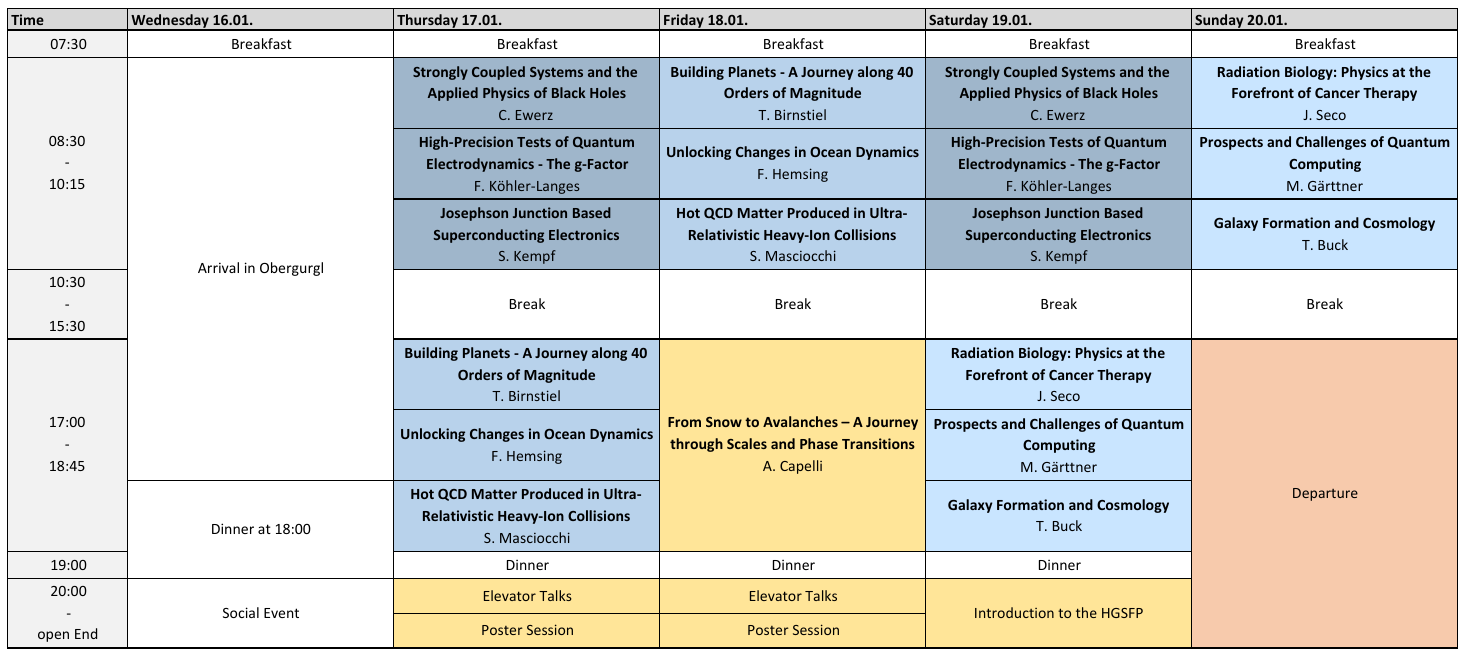
\includegraphics[scale=0.66, angle = 90 ]{figures/Program.jpg}
\end{figure}


\section*{B $\qquad$ Evaluation}

\newpage